\documentclass[11pt]{report}
\setlength{\headheight}{14pt}

\usepackage[a4paper, hmargin=2cm, vmargin=3cm]{geometry}
\usepackage[skip=11pt]{parskip}

\usepackage[T1]{fontenc}

\usepackage{hyperref}
\hypersetup{
    colorlinks=true,
    linkcolor=blue,
    filecolor=magenta,
    urlcolor=blue,
    bookmarksopen=true,
    pdftitle={Northport Manual}
}

\usepackage{enumitem}
\setitemize{noitemsep}

\usepackage{tikz}
\usetikzlibrary{positioning}
\usetikzlibrary{arrows.meta}

\usepackage{titlesec}
\titleformat{\chapter}[hang]
    {\Huge\bfseries}
    {Chapter \thechapter\hspace{4pt}{|}\hspace{20pt}}
    {0pt}
    {\Huge\bfseries}

\usepackage{fancyhdr}
\pagestyle{fancy}
\fancyhf{}
\lhead{\leftmark}
\rfoot{Northport Manual}
\lfoot{Page \thepage}

\title{Northport Manual}
\author{Dean T, Northport Contributors}

\newcommand{\chapterpage}[1]{
    \pagestyle{empty}
    \chapter{#1}
    \newpage
    \pagestyle{fancy}
}

\newcommand{\drawlogo}{
    
\begin{tikzpicture}[baseline]
    \fill[black, draw=black] (2, 3) -- (5, 1) -- (5, 0) -- cycle;
    \fill[white, draw=black] (2, 3) -- (4, 0) -- (5, 0) -- cycle;
    \fill[black, draw=black] (8, 3) -- (6, 0) -- (5, 0) -- cycle;
    \fill[white, draw=black] (8, 3) -- (5, 1) -- (5, 0) -- cycle;
    \fill[black, draw=black] (8, -3) -- (5, -1) -- (5, 0) -- cycle;
    \fill[white, draw=black] (8, -3) -- (5, 1) -- (5, 0) -- cycle;
    \fill[black, draw=black] (2, -3) -- (5, 1) -- (5, 0) -- cycle;
    \fill[white, draw=black] (2, -3) -- (6, 0) -- (5, 0) -- cycle;

    \fill[black, draw=black] (0, 0) -- (4, 1) -- (5, 0) -- cycle;
    \fill[white, draw=black] (0, 0) -- (4, -1) -- (5, 0) -- cycle;
    \fill[black, draw=black] (5, 5) -- (6, 1) -- (5, 0) -- cycle;
    \fill[white, draw=black] (5, 5) -- (4, 1) -- (5, 0) -- cycle;
    \fill[black, draw=black] (10, 0) -- (6, -1) -- (5, 0) -- cycle;
    \fill[white, draw=black] (10, 0) -- (6, 1) -- (5, 0) -- cycle;
    \fill[black, draw=black] (5, -5) -- (4, -1) -- (5, 0) -- cycle;
    \fill[white, draw=black] (5, -5) -- (6, -1) -- (5, 0) -- cycle;
    \end{tikzpicture}
}

\begin{document}
\raggedright

\pagestyle{empty}
\pagenumbering{gobble}


\begin{titlepage}
    \begin{flushleft}
    \vspace{1cm}
    \Huge
    \textbf{Northport Manual}

    \rule{\textwidth}{2pt}
    \large
    Documentation for the kernel and supporting libraries.

    \vspace{4cm}
    \Large
    \center{\textit{N\hspace{-0.33em}P}}
    \center{\drawlogo}
    \vfill
    
    \begin{flushright}
    \small
    by
    \large
    \textbf{Dean T, Northport Contributors}
    
    \normalsize
    \today
    \end{flushright}

    \end{flushleft}
\end{titlepage}

\newpage
\newgeometry{vmargin=2cm, hmargin=4cm}
{
    \hypersetup{linkcolor=black}
    \tableofcontents
}
\restoregeometry
\newpage
\pagenumbering{arabic}
\pagestyle{fancy}

\chapterpage{Introduction}
\section{Preamble}
First of all, thanks for taking an interest in the project! If you're somehow reading this without a copy of the source code, there are copies hosted at the following sites:

\begin{itemize}
    \item Codeberg: \url{https://codeberg.org/r4/northport}
    \item GitHub: \url{https://github.com/deanoburrito/northport}
\end{itemize}

If you encounter any bugs or issues, feel free to open an issue on either of the repository mirrors listed above. If you just want to chat about the project the best way is on discord (\verb|r4#8873|).

\section{Contributors}
While git tracks contributors to the project, there has been a few rewrites over time, so for posterity a complete list of all contributors is maintained here. 

\begin{itemize}
    \item Dean T, \url{https://github.com/deanoburrito}
    \item Ivan G, \url{https://github.com/dreamos82}
\end{itemize}

\section{References \& Thanks}
I wanted to say a personal thanks to the following projects and resources, and the authors behind them, as they've helped me at various points throughout the development of northport. Any code from these projects has been licensed as appropriate, while some have been useful as a point of comparison, or helpful in understanding new concepts.

\begin{itemize}
    \item The Limine Bootloader: \url{https://github.com/limine-bootloader/limine}
    \item Nanoprintf: \url{https://github.com/charlesnicholson/nanoprintf}
    \item Qoi (Quite Ok Image) Format: \url{https://github.com/phoboslab/qoi}
    \item Frigg Utils Library: \url{https://github.com/managarm/frigg}
    \item Luna Hypervisor: \url{https://github.com/thomtl/Luna}
    \item SCAL-UX: \url{https://github.com/NetaScale/SCAL-UX}
    \item Ironclad: \url{https://www.nongnu.org/ironclad/}
    \item MentOS: \url{https://github.com/mentos-team/MentOS}
\end{itemize}

The builtin terminal font is \href{https://github.com/viler-int10h/vga-text-mode-fonts/blob/master/FONTS/NON-PC/APRIXENC.F14}{APRIXENC.F14} from \href{https://github.com/viler-int10h/vga-text-mode-fonts}{this collection} of x86 text mode fonts.

\section{License}

The source for this manual and all compiled copies fall under the same MIT license as the rest of the project. For completeness, a copy is embedded below:

\begin{verbatim}
MIT License

Copyright (c) Dean T.

Permission is hereby granted, free of charge, to any person obtaining a copy
of this software and associated documentation files (the "Software"), to deal
in the Software without restriction, including without limitation the rights
to use, copy, modify, merge, publish, distribute, sublicense, and/or sell
copies of the Software, and to permit persons to whom the Software is
furnished to do so, subject to the following conditions:

The above copyright notice and this permission notice shall be included in all
copies or substantial portions of the Software.

THE SOFTWARE IS PROVIDED "AS IS", WITHOUT WARRANTY OF ANY KIND, EXPRESS OR
IMPLIED, INCLUDING BUT NOT LIMITED TO THE WARRANTIES OF MERCHANTABILITY,
FITNESS FOR A PARTICULAR PURPOSE AND NONINFRINGEMENT. IN NO EVENT SHALL THE
AUTHORS OR COPYRIGHT HOLDERS BE LIABLE FOR ANY CLAIM, DAMAGES OR OTHER
LIABILITY, WHETHER IN AN ACTION OF CONTRACT, TORT OR OTHERWISE, ARISING FROM,
OUT OF OR IN CONNECTION WITH THE SOFTWARE OR THE USE OR OTHER DEALINGS IN THE
SOFTWARE.
\end{verbatim}

\section{Target Audience}
If you're reading this, you're probably the target audience. An intermediate level of C++ knowledge is expected, as is familiarity with working in a freestanding environment.

The purpose of this manual is document northport's design and implementation; not any of the hardware or protocols it may interact with. Descriptions of things external to the project will only be provided if necessary for another explanation.
Having said that, if you find something lacking or that could use clarification, feel free to let me know, or open a PR!

\section{Roadmap}
An up-to-date roadmap is kept in the source directory, at \verb|docs/roadmap.md|. This is where overall progress is tracked, broken down into individual features. Plans for future features are here too, but these will likely change over time.

A quick summary of the current features is also available in the project's readme, available in the root directory.

\section{Terminology}
Where possible, standard terminology is used to keep things accessible, but there are some less-standard terms and concepts used. For completeness they're described here:

\begin{itemize}
    \item \textbf{HHDM}: Higher Half Direct Map, a term borrowed from the Limine bootloader, this refers to an identity map of all physical memory that has been offset into the higher half. An identity map allows you to access physical memory at the same virtual address, and the HHDM works in a similar way but a fixed offset is added to the virtual address. This allows a full memory of physical memory to be accessible without impacting the lower half. The two fields used to manage this in the kernel (\verb|hhdmBase| and \verb|hhdmLength|) are determined once when the kernel is booted and are constant through the kernel's lifecycle. These values will only change when the kernel is booted, and are otherwise constant throughout it's lifetime. 
    \item \textbf{SUMAC}: A portmanteau of SUM (a riscv term) and SMAP (an x86 term), retconned to mean Supervisor/User Memory Access Control. SUMAC is enabled by default on systems where it's supported, and prevents the kernel from unintentionally accessing user memory. This feature is temporarily disabled when copying data in/out of the kernel address space during system calls, and otherwise is on at all times.
    \item \textbf{Extended Registers}: This term refers to any non-integer registers present in a processor. The kernel will always preserve integer registers on entry and exit, but extended registers are preserved lazily. Typically this is any floating point and vector registers that are present.
\end{itemize}

\section{Build System}
\label{Build System}
The entire project is built using GNU make, core utils and some platform-specific deployment tools. 

\subsection{Requirements}
\begin{itemize}
    \item GNU Make.
    \item Core utils (rm, mkdir, cp and friends).
    \item A cross compiler: GCC and clang are both supported.
    \item Xorriso.
    \item \href{https://github.com/limine-bootloader/limine}{The limine bootloader}. A binary release is fine, no need to build from source. See their instructions for how to download and install the latest release.
    \item A system root for the target platform. GCC cross compilers include this, clang does not and you will need to source your own.
\end{itemize}

The project is built as a series of smaller sub-projects, each living in their own directory. The root makefile combines a user config file (\verb|Config.mk|) and config file specific to the target platform (\verb|misc/cross/xyz/CrossCronfig.mk|) and populates some variables for compilation. These variables include compiler and linker flags, the toolchain binaries themselves, and how the final file should be presented (as an iso, or a plain kernel elf, depending on the target's requirements).

When a subproject is built, the root makefile recursively calls \verb|make| inside the project directly, and exports the previously created variables. Each subproject then builds itself, making use of the provided compiler flags and co.

The root makefile can be thought of as a glorified config mechanism, provoding settings to each subproject. The subproject's makefile then provides the scaffold of how to actually build the subproject, and the scaffold is filled in by the variables from the root makefile.

There are some additional files \verb|misc/BuildPrep.mk| and \verb|misc/RunDebug.mk| which provide useful functionality for interacting with the project, but are not directly related to building. \verb|RunDebug.mk| provides make targets for launching and debugging the kernel inside of qemu, and \verb|BuildPrep.mk| converts the user-facing options into compiler flags and pre-processor definitions.

\paragraph{Target Triplets}
The project currently uses the reduced versions of target triplets in the form of \verb|elf-$(ISA)|, where \verb|$(ISA)| is the target instruction set. As an example, this means any riscv64 platforms would use the target triplet \verb|elf-riscv64|, regardless of their ISA string (riscv64gcv for example). For x86\_64 the target triplet is \verb|elf-x86_64|.

In practice, target triplets are used to select toolchain binaries used for GCC, and given as the \verb|--target=| parameter for clang.

\paragraph{Libraries}
So far only a single library exists, but more are planned. Common make rules and targets are defined in a separate file (\verb|misc/LibCommon.mk|) which can then be included into a library's makefile. This is to save duplicating common build code across all libraries.

\paragraph{Kernel Syslib}
The \verb|np-syslib| library is actually built twice: once with the usual flags, and a second time with kernel-appropriate flags. The kernel version (\verb|knp-syslib|) is linked with the kernel, and has more restrictions placed on the code generation (for example, it only uses integer registers). Other programs and libraries are free to use the kernel version of np-syslib, and while there is no harm in doing so it is not recommended due to the extra restrictions placed on kernel code.

\subsection{Configuration}
Configuration is done in two places: at a global level in \verb|Config.mk|, and at a platform-specific level in \verb|misc/xyz/CrossConfig.mk|, where xyz is the target platform.

The global config is where you can set the cross-compiler paths, select the compiler you want to use and other common options like your target platform. The available options are documented in the config file itself.

Each supported platform has it's own \verb|CrossConfig.mk| file, where some platform specific compiler and linker flags can be set (like the codemodel). Other actions can be taken here as well, like changing the default build target. The available options are described below.

\begin{itemize}
    \item \verb|KERNEL_CXX_FLAGS|: This variable contains all the C++ compiler flags used for the kernel. Only platform-specific flags should be added here, for flags that affect all platforms add them in \verb|Config.mk|.
    \item \verb|KERNEL_LD_FLAGS|: For adding to the kernel linker flags, similar to the above option.
    \item \verb|ARCH_DEFAULT_TARGET|: Sets the makefile target to be used for \verb|make all|. Different platforms may require the kernel/system to be in different formats, UEFI systems accept a bootable iso for example. Some other systems may only support the bare kernel binary. Currently two builtin targets are provided: \verb|binaries| just compiles the kernel binary, and \verb|iso| which creates a UEFI iso with limine and the kernel.
    \item \verb|QEMU_BASE|: Base flags and the qemu binary to use.
    \item There are some other \verb|QEMU_*| flags that are added to the base flags depending on which make target is used (KVM/no KVM, UEFI/no UEFI).
\end{itemize}

\subsection{Make Targets}
The following make targets are available in the root makefile (i.e. from the project root directory). This is the intended interface into the build system.

While GNUmake is used for the build system, northport \textbf{does not} make use of dependency files (\verb|.d|) currently, so changes to \verb|.cpp| source files will trigger a rebuild of that file, changes to a \verb|.h| header file will not trigger rebuilds in affected source files. To test changes made to a header file, the recommended approach is to run \verb|make clean| followed by \verb|make| to perform a clean rebuild.

\begin{itemize}
    \item \verb|make|: Prints the help text, showing a summary of available make targets and notable files.
    \item \verb|make all|: Performs an incremental build of everything, and then performs a platform-specific packaging step. This might include burning a bootloader to an iso file, or leaving the kernel binary as is.
    \item \verb|make clean|: Completely removes all build files, resulting in the next build starting from scratch.
    \item \verb|make run|: Creates a platform-specific package, and launches it in qemu for the target architecture. By default this tries to use KVM.
    \item \verb|make run-kvmless|: Same as above, but explicitly disables use of KVM.
    \item \verb|make debug|: Similar to \verb|run|, but halts the virtual machine and starts the qemu gdb server with default arguments.
    \item \verb|make attach|: The other half of \verb|debug|, launches gdb with the kernel symbols loaded, and attempts to connect the qemu gdb server (default settings: tcp/1234).
    \item \verb|make docs|: Renders the documentation as a pdf.
    \item \verb|make docs-clean|: Removes temporary build files related to docs, useful after updating latex toolchain or a buggy build.
\end{itemize}

\subsection{Development Cycle}
For the initial setup you'll need to clone the repository, install any missing tools from the list above, and then adjust the global config (\verb|Config.mk|) to suit your environment. After opening a shell in the project root directory, and executing \verb|make run| the project should build and qemu should launch with the kernel. If this works then you're good to go.

General development is straightforward, \verb|make run| can be used to build the latest changes and test them. If you need to debug you can use \verb|make debug| in one terminal to launch qemu and \verb|make attach| in another to launch and attach gdb. As mentioned previously header files are not tracked as dependencies, so a clean build may be required when editing those.

Performing a clean build is also required when changing the target architecture, as the ISA the file was compiled for is not tracked. If a clean build is not performed you may encounter linker errors.

\section{Project Layout}
At the root level, the kernel and initdisk sources are available as separate directories, alongside \verb|libs/| which contains project directories for any support libraries.

The \verb|initdisk/| directory contains files used to build the initial ramdisk, which houses non-critical but nice-to-have files for the kernel. This subproject can contain all kinds of assets, not just source code.

The \verb|kernel/| source tree roughly shows the various kernel subsystems. For example the \verb|kernel/cpp/| directory contains code required to support some C++ language features, like the stack protector implementation, program sanitizers or stub functions required to be implemented by the C++ standard. The \verb|kernel/config/| directory contains code used for detecting the configuration of the current system, and so on.

The kernel also contains an \verb|kernel/arch/| directory, which is special. Only \textit{one} of the subdirectories is included when building the project. The name of the included subdirectory is derived from the target architecture of the compilation. As an example, if the kernel is being built for riscv64, only \verb|kernel/arch/riscv64| is included in the compilation process, not \verb|kernel/arch/x86_64| or any other architecture folder. This logic also applies to the include paths used for headers.

All subprojects that provide header files will make them available under an \verb|include/| directory inside the subproject's root directory.

Most projects will store build-artefacts under a \verb|build/| directory within their subproject folder. The \verb|build/| directory is purged on a clean build, and it's contents shouldn't be relied upon for anything other than potentially reducing compile times.

\subsection{Documentation}
As you might expect, the \verb|docs/| directory contains files related to documentation. The top level contains a handful of files like the project roadmap, and basic build instructions for those who don't want to (or cant) build the documentation.

The \verb|docs/manual/| directory contains the \LaTeX \hspace{0.25em}source for building this document, organised into relevant chapters.

Project imagery is also stashed in \verb|docs/images/|. This \textbf{does not} mean screenshots (which are stored external to the git repository) but rather banners and icons for use in the documentation.

\subsection{Miscellanious}
The \verb|misc/| directory contains a few things. Binary assets for the built-in terminal are stored here (\verb|misc/TerminalFont|, and optionally \verb|misc/TerminalBg.qoi|). Utility makefiles are also kept here (\verb|RunDebug.mk|, \verb|BuildPrep.mk|, and \verb|LibCommon.mk|), see \autoref{Build System} for how these are used.

Target-specific compilation files are also stored here, under \verb|misc/cross/|. Each target is given a separate subdirectory containing a \verb|CrossConfig.mk| which is used to augment the build system when targetting this platform. Other platform-specific files may be stored here, like bootloader configuration (\verb|limine.cfg|).


\chapterpage{Kernel}
\section{Overview}
Northport is a monolithic kernel, with some modularity planned for later drivers. The kernel is booted via the limine boot protocol, and begins with some platform specific initialization. After this the clock and scheduler are started, and then the kernel operates as series of \textit{mostly} independent subsystems. The exceptions being the scheduler and virtual memory subsystem as most parts of the kernel will interact with these.

The kernel makes full use of multi-processor systems, and can run with minimal memory requirements.

\subsection{Kernel Subsystems}
\begin{itemize}
    \item Memory: physical memory manager, virtual memory managers, kernel heap.
    \item Tasking: software clock, scheduler, threads and processes.
    \item Hardware abstraction: functionality required from the underlying hardware that cannot be provided by a driver. Things like the IPI mechanism used and interrupt management are handled here.
    \item Filesystems: VFS, and filesystem drivers.
    \item Debugging: logging facilities, built-in graphical terminal.
    \item Hardware discovery: ACPI table parsing, PCI device enumeration, device tree parsing.
    \item Driver and Device management: Loading, starting and stopping drivers in response to system events like hardware discovery.
\end{itemize}

There are some other minor subsystems like interrupt vector allocation and IPI mailboxes for communicating on multi-core systems.

\subsection{Init Sequence}
The philosophy of the entry sequence for the kernel is to allow the platform core to contain the messy parts required to interface with hardware, and call various hooks for generic parts of the init sequence when appropriate for the platform. Each architecture contains a \verb|arch/xyz/Init.cpp| file with a few common functions. These functions are not required, but are named this way for consistency.

\begin{itemize}
    \item \verb|KernelEntry()|: This is where the first core starts executing the kernel. This function is usually the ELF entry point, unless the limine boot shim is active. This function does any early set up the platform might require, and then enables the memory subsystems, early platform subsystems (logging), timing subsystem and then performs any core-local set up for BSP (a term borrowed from x86). 
    \item \verb|ApEntry()|: APs (borrowed from x86) require a different codepath to the BSP, and this function is where they begin executing. Most of the time this is just calling \verb|InitCore()|.
    \item \verb|InitCore()|: This function is either called by \verb|KernelEntry()| or \verb|ApEntry()| and performs any initialization required for each processor core in the system. This includes allocating and populating the core-local block, and setting any supported feature flags.
\end{itemize}

\subsubsection{Platform-Independent Init}
The file \verb|CommonInit.cpp| contains initialization code that needs to happen across all platforms. These are provided as hooks that the platform-specific init code can call when it's ready. These hook functions should be called in order.

\begin{itemize}
    \item \verb|InitEarlyPlatform()|: This should be called as early as possible. Here bootloader data is verified to be sane, and the HHDM base and length are determined. Early outputs for logging are detected here, namely a bootloader-provided framebuffer and serial devices.
    \item \verb|InitMemory()|: Initializes the physical memory manager, virtual memory manager and the kernel heap.
    \item \verb|InitPlatform()|: Hardware discovery methods are initialized here (ACPI tables and/or the DTB are parsed). Some global kernel state is also initialized like the core-independent part of the scheduler and interrupt vector allocator.
    \item \verb|ExitBspInit()|: Starts the system clock and then calls \verb|ExitApInit()| (see below).
    \item \verb|ExitApInit()|: Sets up the IPI mailbox for the core, decreases a reference count to bootloader data and then begins scheduled execution. If the reference count is decremented to 0, the core will launch a thread that reclaims bootloader memory and makes it available to the physical memory manager.
\end{itemize}

\begin{figure}[h]
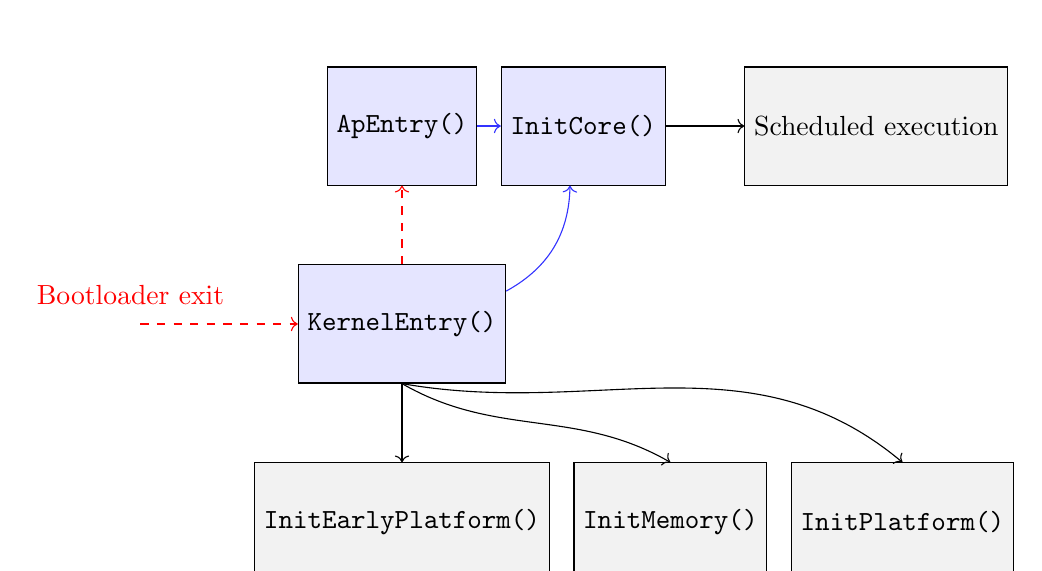
\begin{tikzpicture}
    \node (ApEntry) [rectangle, minimum height=1.5cm, draw=black, fill=blue!10] {
        \verb|ApEntry()|};
    \node (KernelEntry) [rectangle, minimum height=1.5cm, draw=black, fill=blue!10, below = of ApEntry] {
        \verb|KernelEntry()|};
    \node (hidden) [left = 2cm of KernelEntry] {};
    \node (InitCore) [rectangle, minimum height=1.5cm, draw=black, fill=blue!10, right = 3mm of ApEntry] {
        \verb|InitCore()|};
    \node (SchedulerExec) [rectangle, minimum height=1.5cm, draw=black, fill=gray!10, right = of InitCore] {
        Scheduled execution
    };
    \node (InitEarlyPlatform) [rectangle, minimum height=1.5cm, draw=black, fill=gray!10, below = of KernelEntry] {
        \verb|InitEarlyPlatform()|};
    \node (InitMemory) [rectangle, minimum height=1.5cm, draw=black, fill=gray!10, right = 3mm of InitEarlyPlatform] {
        \verb|InitMemory()|};
    \node (InitPlatform) [rectangle, minimum height=1.5cm, draw=black, fill=gray!10, right = 3mm of InitMemory] {
    \verb|InitPlatform()|};

    \path [->, red, dashed] (hidden) edge (KernelEntry.west) node [label=above:Bootloader exit]{};
    \path [->] (KernelEntry.south) edge (InitEarlyPlatform);
    \path [->, in=150, out=-30] (KernelEntry.south) edge (InitMemory.north);
    \path [->, in=140, out=-10] (KernelEntry.south) edge (InitPlatform.north);
    \path [->, red, dashed] (KernelEntry) edge (ApEntry);
    \path [->, bend right, blue!80] (KernelEntry) edge (InitCore);
    \path [->, blue!80] (ApEntry) edge (InitCore);
    \path [->] (InitCore) edge (SchedulerExec);
\end{tikzpicture}

\centering
\begin{tabular}{c|c|l}
    \begin{tikzpicture}
        \path [->, red, dashed] (0, 0) edge (1, 0);
    \end{tikzpicture} 
    & 
    & Platform-specific mechanism. \\

    \begin{tikzpicture}
        \path [->, blue!80] (0, 0) edge (1, 0);
    \end{tikzpicture} 
    & 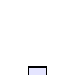
\begin{tikzpicture} \node (r)[rectangle, draw=black, fill=blue!10] (0, 0){}; \end{tikzpicture} 
    & (Call to) platform specific code. \\

    \begin{tikzpicture}
        \path [->, black] (0, 0) edge (1, 0);
    \end{tikzpicture} 
    & 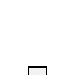
\begin{tikzpicture} \node (r)[rectangle, draw=black, fill=gray!10] (0, 0){}; \end{tikzpicture}
    & (Call to) common init code. \\
\end{tabular}
\caption{Kernel operation pre-scheduler.}
\end{figure}

\subsection{Multi-Core Systems}
The kernel is written and tested with multi-core systems in mind, but it's also capable of running on single-core systems. 

From the perspective of the kernel, each core operates independently of the others. The majority of the kernel subsystems are unaware of how many cores are present in the system. The scheduler and IPI mailboxes are the notable exceptions, as they operate on a per-core basis. The scheduler is covered in more in \autoref{Scheduler}.

During initialization one core is considered the boot core (the BSP, to use the x86 term) and will set up the initial memory management structures used for the kernel, and perform other early init operations like discovering and initializing early log outputs (like serial devices or the bootloader framebuffer). The boot core is also responsible for starting the other cores in the system so they can initialize themselves. Once each core has finished initializing itself, it will begin scheduled execution. 

At runtime one core is given the special duty of managing the system clock. This is often the boot core, but is not required to be. The clock core is responsible for managing the hardware timer(s) used to provide the clock functions to the rest of the kernel.

If for some reason a function is required to run on a specific core, there are two options:
\begin{itemize}
    \item A thread can be created to run the function, and pinned to a specific core. This is the recommended approach for code without timing requirements.
    \item Each core has an IPI mailbox. Each mail item consists of a function pointer and an argument to pass to the function when run. When mail is sent the target core is sent an IPI and the function will whenever the IPI is served. See the function \verb|SendIpiMail()| in \verb|interrupts/Ipi.h|.
\end{itemize}

\subsubsection{Example Code}
To use the mailbox mechanism all that's required a pointer to the function to run on the remote core. In the example we'll assume core 5 exists and we want to run \verb|ExampleFunction()| on that core. The callback function can optionally have an argument passed to it at runtime, but it's not required so we'll use \verb|nullptr|. We omit the argument in this example. The function we'll use is defined in \verb|interrupts/Ipi.h|.

\begin{verbatim}
void ExampleFunction(void* ignored);

SendIpiMail(5, ExampleFunction, nullptr);
\end{verbatim}

\section{Supported Platforms}
This version of the kernel was written with support for multiple platforms in mind from the beginning, and it was one of the earliest features of the kernel. Currently only two platforms are supported (x86\_64 and riscv64) but it would be nice to add more in the future, namely aarch64 and perhaps something more exotic.

The current platforms and their status are listed below.

\begin{tabular}{|r|l|p{0.3\linewidth}|p{0.4\linewidth}|}
    \hline
    \textbf{Platform} & \textbf{Qemu} & \textbf{Hardware} & \textbf{Notes} \\
    \hline
    x86\_64 & Yes & 3 machines tested, 2 work. & \\
    riscv64 & Yes & No & Support for a visionfive-2 port is planned once some bugs are ironed out in the virtio machine.\\
    \hline
\end{tabular}

\subsection{Platform Abstraction Layer}
The kernel maintains a strict boundary between platform-specific code and platform-independent code. The platform specific code is contained within the \verb|kernel/arch/xyz| and \verb|kernel/include/arch/xyz| directories, where \verb|xyz| is the target architecture. Each platform is given it's own directory, and the layout inside this directory can be considered freeform.

Each platform \textbf{must} implement the functions defined in each header file under \verb|kernel/include/arch|. These headers contain functions required by the rest of the kernel. Code within an arch directory is allowed to include headers from within it's own \verb|include/arch/xyz/| directory, however all other kernel code is only permitted to use the generic headers found in \verb|include/arch/|.

\subsubsection{Platform.h}
This file is a special case, as the platform agnostic \verb|kernel/include/arch/Platform.h| provides some complete definitions (like the core-local data struct), some utility functions and also some function declarations. These declarations serve as a guide for what a platform would need to implement to support a port of the kernel. 

Most of the declared functions can be implemented by simple inline assembly, and often these functions are made \verb|inline| (often with \verb|[[gnu::always_inline]]| too). There are some additional constants that must be defined within an implementation of this header:

\begin{itemize}
    \item \verb|size_t PageSize|: The native page size of the target platform, in bytes. Most platforms will have this as 4K (0x1000) bytes.
    \item \verb|size_t IntVectorAllocBase|: Used by the interrupt vector allocator, this sets the lowest vector number available for general use. Vectors will never be allocated below this.
    \item \verb|size_t IntVectorAllocLimit|: Largest interrupt vector allowed to be allocated (inclusive). Set this and \verb|IntVectorAllocBase| to 0 to disable the vector allocator and the ability to install interrupt handlers.
\end{itemize}

Of course platforms are free to define their own internal constants here too, for example x86\_64 defines a number of MSR and port values.

\subsection{Platform Requirements}
The northport kernel is inteded to run on mobile or desktop class processors, and currently there is no intent to support embedded processors.

The hardware requirements for adding a new platform are described below.

\begin{itemize}
    \item An MMU for managing the virtual address space, with the ability to distinguish between supervisor and user levels, and r/w/x access control.
    \item Basic interrupt architecture: sending device interrupts to specific processors, or at least limiting which processors can receive them. The ability to send IPIs is also required on multi-core systems.
    \item A single timer capable of sending an interrupt on a terminal count (one-shot operation), and a timer that can be used for polling. There are no strict timing requirements, but the kernel internally tracks time as nanoseconds, and so it can make use of more precise timers if available. The kernel doesn't care if these two functions are provided by the same piece of or hardware or two separate pieces. Only one of each type of timer is needed, and they both need to be accessible from the same processor. The system must provide a way to calibrate each timer.
    \item The kernel expects to be booted in accordance with the Limine Boot Protocol. If a compatible bootloader exists for the target platform that's easy, but if not the boot shim included in the kernel may need to be modified.
\end{itemize}

The kernel also has a soft requirement of being running on a 64-bit processor. Although it should be possible to port to a 32-bit system, this isn't a goal of the project and is yet to be tested.

\section{Limine Protocol Shim}
The northport kernel is booted via the limine boot protocol (LBP), normally provided by the Limine Bootloader. Unfortunately the bootloader only supports aarch64 and x86 platforms for now, for a solution is needed for booting on riscv: a boot shim that understands the boot protocol.

The shim is an optional chunk of code that is only compiled in when \verb|NP_INCLUDE_LIMINE_BOOTSTRAP| is defined. Some parts of the protocol are also platform-specific, like the SMP feature response and entry machine state and therefore have no official definition for riscv. A tentative version of these is documented down below, as implemented by the boot shim, but please remember these are extentions to the original protocol and only supported by the boot shim, not the original bootloader.

\paragraph{Disclaimer}
The boot shim is a combination of generic and \textit{some} hardware specific code. It's not guarenteed to work on any particular riscv hardware, and currently only has support for the qemu virt board.

In reality this shim is intended as a temporary solution until EFI on riscv is more usable, and a proper bootloader can be written or ported over. 

\subsection{Supported Features}
While the shim supports the limine boot protocol, it targets the northport kerenl in particular. The kernel only *requires* the kernel address, memory map and hhdm feature responses, but *can* make use of others. The shim knows this and may not support any other features depending on the particular hardware. 

This is allowed in the original LBP specification, as bootloaders are recommended to ignore feature tags they don't recognise.

\subsection{Why Use LBP At All?}
Since early boot code was going to need to be written for a new platform anyway, there were considerations of coupling it directly to the kernel; removing limine from the boot sequence entirely.

Ultimately this was decided against as the protocol provides a nice abstraction to the parts of the kernel that use it. A quick test of the protocol resulted in duplicating a lot of the work already done, and that was messy.

In a more altruistic light, hopefully this early work on LBP on riscv can be useful to porting the official bootloader in the future.

\subsection{Internals}
\textit{For now, the internals of the boot shim remain undocumented as it's quite messy and will likely undergo a huge rewrite soon. If you have questions it's best to contact me directly.}

\subsection{Current Protocol Extensions}
As previously mentioned, architecture specific parts of the specificiation are undefined for riscv platforms and we've synthesized our interpretation of a sane entry machine state and SMP feature response. Again please note that this is not official, and may change if the original protocol is ported.

\paragraph{Risc-V Entry Machine State}
The \verb|pc| register will point to the declared entry function, unless an entry point feature is requested then the value of \verb|pc| is taken from there. \textit{Authors note: the shim currently ignores this and instead always jumps to KernelEntry(), which would normally be the entry point for the kernel.} The kernel is entered from supervisor mode.

Supervisor interrupts are mased in \verb|sstatus.sie| and \verb|sie| (appropriate bits are cleared). The contents of \verb|stvec| are undefined. Supervisor access to user memory is disabled (\verb|sstatus.sum| is cleared), make-executable-readable is also disabled (\verb|sstatus.mxr| is cleared).

Paging is enabled, with mappings compatible with the page map described earlier. The contents of \verb|satp| and the page tables are undefined, but the page tables are guarenteed to be in bootloader-reclaimable memory. \textit{TODO: satp.mode? what guarentees do we make about that?}

A stack is setup, located in bootloader-reclaimable memory, of at least 64KiB in size, or the value specified in a stack size request. All general integer registers are zero. If they exist, extension registers (floating point, vector) and related CSRs are in an undefined state.

EFI boot services are exited.

\paragraph{Risc-V SMP Feature Response}
The request for this feature is identical to the base version, how the response struct and per-core structs differ. Their definitions are below.

\begin{verbatim}
struct limine_smp_info {
    uint64_t hart_id;
    uint32_t context_id;
    uint32_t reserved;
    limine_goto_address goto_address;
    uint64_t extra_argument;
};

struct limine_smp_response {
    uint64_t revision;
    uint64_t bsp_hart_id;
    uint64_t cpu_count;
    limine_smp_info** cpus;
};
\end{verbatim}

Most of the fields should be familiar except the \verb|context_id|, which contains the integer used by interrupt devices to represent supervisor interrupts on a particular hart. This is required to properly use devices like the PLIC or IMSIC. 

\section{Physical Memory Manager}
The kernel uses a relatively simple physical memory manager design, with a focus on keeping allocations fast and using granular locking to reduce contention between multiple cpus trying to allocate at the same time.

A bitmap allocator is not the fastest, but it is accountable. This is an important feature in the PMM design: bad attempts to free physical memory won't result in corrupt state. While other allocator designs can offer this, a bitmap is simple to implement.

\subsection{Concepts}
\paragraph{PM Zone}
Zones are used to arbitrarily section-off parts of physical memory. In northport two zones are used: the low zone (32-bit addressable memory), and the high zone (addresses > 4GiB).
This is done in an attempt to preserve 32-bit addressable memory for older devices that only support these 32-bit addresses. While these devices are less common, they are not extinct.

\paragraph{PM Range}
A range represents a number of contiguous physical pages, and tracks the state of each page (used/free) in a bitmap. A range also contains some metadata like where the next free page is, the total number of free and used pages, etc. Each range is responsible for a fixed number of pages, but the PMM's view of physical memory can be modified by adding or removing ranges.

As the ideas of a range or zone are used elsewhere in the kernel, these are referred to as \textbf{PM}Ranges or \textbf{PM}Zones to indicate they represent physical memory.

\begin{figure}[h]
\centering
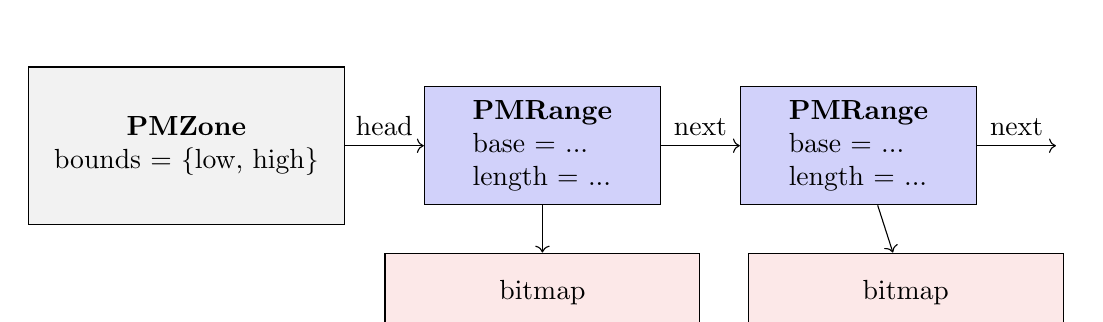
\begin{tikzpicture}
    \begin{scope}
    \node (1) [rectangle, minimum width=3cm, minimum height=2cm, draw=black, fill=gray!10] {
        \begin{tabular}{c}
            \textbf{PMZone} \\
            bounds = $\lbrace$low, high$\rbrace$
        \end{tabular}};
    \node (2) [rectangle, minimum width=3cm, minimum height=1cm, draw=black, fill=gray!20!blue!20, right = of 1] {
        \begin{tabular}{l}
            \textbf{PMRange} \\
            base = ... \\
            length = ... \\
        \end{tabular}};
    \draw [->] (1) -- node[above] {head} (2);
    \node (3) [rectangle, minimum width=3cm, minimum height=1cm, draw=black, fill=gray!20!blue!20, right = of 2] {
        \begin{tabular}{l}
            \textbf{PMRange} \\
            base = ... \\
            length = ...
        \end{tabular}};
    \draw [->] (2) -- node[above] {next} (3);
    \node (4) [right = of 3] {};
    \draw [->] (3) -- node[above] {next} (4);
    \end{scope}
    \begin{scope}[node distance=6mm]
        \node (bitmap0) [rectangle, minimum width=4cm, minimum height=1cm, draw=black, fill=gray!20!red!10, below = of 2] {bitmap};
        \node (bitmap1) [rectangle, minimum width=4cm, minimum height=1cm, draw=black, fill=gray!20!red!10, right = of bitmap0] {bitmap};
        \draw [->] (2) -- (bitmap0);
        \draw [->] (3) -- (bitmap1);
    \end{scope}
\end{tikzpicture}
\caption{Relationship between PMZones and PMRanges.}
\end{figure}

\begin{figure}[h]
\centering
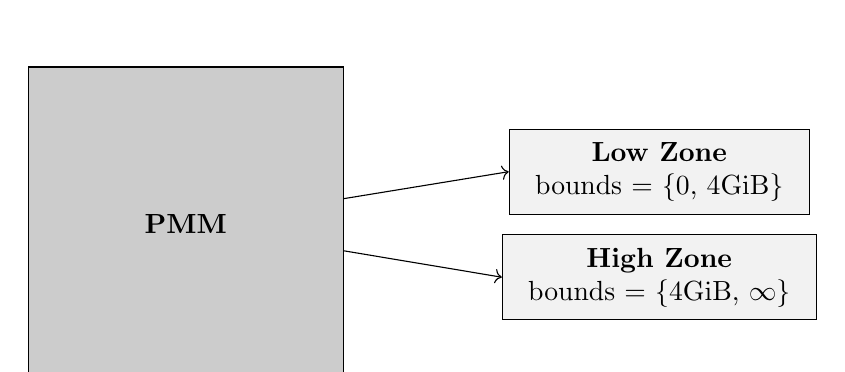
\begin{tikzpicture}
    \node (pmm) [rectangle, minimum width=4cm, minimum height=4cm, draw=black, fill=gray!40] {
        \textbf{PMM}
    };
    \node (placeholder) [minimum width=4cm, minimum height=0cm, right = 2cm of pmm]{};
    \node (lowzone) [rectangle, minimum width=2cm, minimum height=1cm, draw=black, fill=gray!10, above = 0mm of placeholder] {
        \begin{tabular}{c} 
            \textbf{Low Zone} \\
            bounds = $\lbrace$0, 4GiB$\rbrace$
        \end{tabular}
    };
    \node (highzone) [rectangle, minimum width=2cm, minimum height=1cm, draw=black, fill=gray!10, below = 0mm of placeholder] {
        \begin{tabular}{c} 
            \textbf{High Zone} \\
            bounds = $\lbrace$4GiB, $\infty\rbrace$
        \end{tabular}
    };
    \draw [->] (pmm) -- (lowzone.west);
    \draw [->] (pmm) -- (highzone.west);
\end{tikzpicture}
\caption{PMM zone configuration.}
\end{figure}

\subsection{Initialization}
The northport PMM uses a bitmap to store the state of page of physical memory. A page is considered the basic unit of the PMM, and it's exact size depends on the target platform and is represented by the constexpr variable \verb|PageSize|.

The first problem the PMM is presented with is finding space for the bitmaps required to manage each region. For memory effeciency these bitmaps are packed together, since the next bitmap can begin inside of the slack space following the previous bitmap. This slack space refers to the space following the end of the bitmap, but before the next page begins. Since the PMM operates in page-sized units, this space is wasted.

The downside to this approach is that a single large space is required for the bitmaps to exist in, rather than many smaller spaces. This is fine on most systems, but may break down on a sufficiency fragmented physical memory map.

The buffer used for the bitmaps is called the \textit{metabuffer} and is also used for allocating the space needed for the PM regions. Each PM region roughly represents a single usable memory map entry. Once the space required for the metabuffer has been calculated, it's length is rounded up to the nearest page and subtracted from the largest memory map entry available before having the hhdm offset added.

The address and length of the metabuffer is stashed, and the PMM begins ingesting each usable memory region from the memory map.

\subsection{Ingesting Memory}
Ingesting physical memory makes it available for use by the rest of the system. Memory can be ingested at any time, although this can become a very expensive operation once more processes are started. While adding memory at runtime is supported, removing memory from the system is currently not.

When memory is ingested it may be split into two separate regions if it crosses a PM zone border. Otherwise the ingested memory is represented by a single PM region. 

The PM regions and their bitmaps are allocated from the metabuffer. Each region is the inserted into the linked list of regions representing the PM zone it's assigned to. This list is sorted by base address (ascending).

At this point the new PM region is live and can be accessed by the rest of the PMM, and can now be used to satify allocations.

\subsection{Allocating Pages}
Allocating memory is very straightforward, each PM region tracks how many free pages it contains. If the region lacks enough free pages to satisfy an allocation request, it's skipped.

Once a region with enough free pages is found, the region's bitmap is scanned until a run of contiguous free pages is found. If this run is not found, the search for a new region with enough free pages continues.

If an allocation request cannot be satisified, the PMM panics the kernel. There are plans to allow the PMM to communicate memory pressure to users of physical memory and request to purge some allocations, allowing physical memory to freed to satisfy other allocations. This (and some other ideas) currently only exist as experiments.

It should be noted that there are two main allocation functions:
\begin{itemize}
    \item \verb|AllocLow()|: This function tries to allocate exlusively from the low zone (< 4GiB), and panics on failure.
    \item \verb|Alloc()|: This function tries to allocate from the higher zone, and on failure calls \verb|AllocLow|. Ultimately this may cause a panic on failure.
\end{itemize}

The intention is for developers to use \verb|Alloc| for general physical memory allocations, and only use \verb|AllocLow| for memory that must be 32-bit addressable.

\subsection{Freeing Pages}
Freeing memory is also straightforward. First the appropriate zone for the allocation is selected, and then the freed address is compared against the base address and length of each PM region in the zone until the matching region is found. If the zone or region could not be determined, an error is logged and the freeing call fails. In this event no bitmap state is modified.

Once the PM region has been located, the corresponding bit is cleared, and the free operation is complete.

Contrary to allocation, there is only a single free function \verb|Free()|.

\subsection{Example Code}
The PMM operates as a singleton, and the global instance is available as \verb|PMM::Global()|. The alloc/free functions will assume a page-count of 1 unless otherwise specified. All the functions used below are declared in \verb|memory/Pmm.h|.

\begin{lstlisting}
uintptr_t singlePage = PMM::Global().Alloc();
uintptr_t sixPages = PMM::Global().Alloc(6);

PMM::Global().Free(singlePage);
PMM::Global().Free(sixPages, 6);
\end{lstlisting}

\section{Heap Allocation}
The kernel heap is provided by a series of aggregate slab allocators and a pool allocator. All of this is hidden behind the heap API, which consists of familiar free/alloc functions, and the C-style \verb|malloc()| and \verb|free()| global functions are provided as well (see \verb|memory/New.cpp|) if they're needed. The C functions are simple wrappers around the main heap functions.

The global \verb|new| and \verb|delete| C++ operators have also been defined, making them available for kernel code. This is the ideal way to manage dynamically allocated memory.

\subsection{Concepts}

\paragraph{Pinned Allocations} By default the kernel heap uses memory that can be swapped (purged from main memory to disk to free memory for use parts of the system) and demand-paged. Allocations can optionally be made \textit{pinned}. Pinned allocations are immediately backed with physical memory and non-swappable, which is useful for critical parts of the kernel infrastructure that can't be swapped out. The container used by the VMM to track allocated VMRanges is an example of when pinned memory is needed. Pinning allocations means that the physical memory used can't be used elsewhere if the system needs it, so they should be used sparingly and only when necessary.

\subsection{Slab Allocators}
For small heap allocations the kernel uses a series of slab allocators, with each slab being 2x the size of the pervious. The smallest slab allocator starts at 32 bytes, and the largest is 512 bytes by default, although this is easily configurable. 

Each slab consists of a number of \textit{slab segments}, which contains a base address and bitmap to track which slabs have allocated relative to the base. A segment also contains some extra metadata to speed up allocations, like hinting at where the last successfull allocation was.

When a segment is full, a new segment is created with identical parameters to the initial segment (slab size and number of slabs). These segments are stored as a linked list, effectively allowing infinite expansion if needed. As each slab tracks the number of free slabs, full segments can quickly be skipped when searching for free space.

\subsubsection{Pinned vs Non-Pinned}
Each slab allocator also tracks if it's pinned or not. Non-pinned slabs operate as you would expect, but pinned slabs are a special exception in how virtual memory is managed in the kernel. There is a circular dependency between pinned slabs and the VMM: since the VMM uses pinned allocations to store its management structures, the slab cannot use the VMM to allocate more virtual address space for itself as this would cause a pinned allocation, and so on. 

The current solution is to reserve an area of virtual memory above the HHDM but below the area the kernel VMM is allowed to allocate in. This area is the same size as the HHDM. A pointer within this area is stored, and is treated like a bump allocator: everytime a pinned slab expands it increments this pointer by the amount of virtual memory the new segment will consume. When it comes to back the new segment with physical memory, the slab modifies the kernel's master page tables directly.

\subsection{Pool Allocators}
The pool allocator is similar to the design of \hyperlink{https://github.com/blanham/liballoc}{liballoc} v1.1. It consists of a number of segments, and each segment is a freelist for a single contiguous block of virtual memory. Over time as the pool allocator expands more segments may be added. 

There are no major differences between the pinned pool vs the non-pinned pool, except for the flags passed to the VMM when requesting virtual memory. The VMM handles the specifics of pinning memory.

\subsection{Example Code}
Like other singleton classes the global kernel heap can be accessed as \verb|Heap::Global()|. All heap declarations are available in the header \verb|memory/Heap.h|. The examples below are for documentation but the built-in C++ operators should be used where possible.

\begin{verbatim}
void* _100Bytes = Heap::Global().Alloc(100);

Heap::Global().Free(_100Bytes);
\end{verbatim}

To use pinned allocations is similar, although you must tell \textit{both} alloc and free that this is pinned memory. This can be done by setting the optional argument to \verb|true|. A \verb|PinnedAllocator| class is also available for use as the allocator argument in template containers.

\begin{verbatim}
void* _40BytesPinned = Heap::Global().Alloc(40, true);

Heap::Global().Free(_40BytesPinned);        //an error
Heap::Global().Free(_40BytesPinned, true);  //okay
\end{verbatim}

\section{Clocks and Timers}
Northport refers to hardware devices that provide timekeeping facilities as timers, and provides a software abstraction on top called a clock. There is only one clock in the system, and the rest of the kernel uses the clock for getting timer callbacks. Internally the clock uses whatever timers are provided by the platform to ensure it can keep the deadlines set by software.

It's important to note that the timing subsystem is 'best-effort' and \textbf{not real time}. Clock events are guarenteed to expire \textit{exactly once}, and \textit{reasonably soon} after their ideal expiry time. Reasonably soon is relative to the accuracy and precision of the hardware timers being used to drive the clock.

\subsection{Hardware Timers}
Northport has very simple timing requirements, this was done with the intent of making the kernel easier to port to other platforms. There are two types of timers we require, although only one of each is necessary.

\paragraph{Polling Timers}
A polling timer only needs to provide a software readable counter. The kernel assumes values returned from the counter increment as time passes, regardless of what the underlying timer does. If the timer counts down, you can return the inverted value (\verb|maxCount - currentCount|). The x86 PIT is one such example, which counts down: and when used for the system polling timer the returned value is inverted so the system sees an incrementing value.

\paragraph{Interrupt Timers}
Interrupt timers require the ability to set a deadline in the future, and generate an interrupt whenthe deadline is passed. Deadlines are often within the 1-1000ms range, but the kernel can take advantage of hardware that supports longer expiry times. Interrupt timers may also be referred to as \textit{sys timers} in the source code (the original term used).

The kernel doesn't interact with the various timers directly, instead it uses the functions defined in \verb|arch/Timers.h| to interface with platform specific code that manages the underlying hardware. Anything beyond the functions in that header are considered implementation details of the platform. This includes calibrating any timers that might require it.

\subsection{Software Clock}
The clock is the main timing interface for the kernel. It works by keeping a list of pending \textit{clock events}. This list is sorted with the soonest event at the head of the list, and each event tracks it's time relative to the previous event. The interrupt timer is set to the first event in the list, and the event's callback function runs is called in response to the timer expiring. The time taken for each callback to run is tracked, and any pending events that would have expired in that time are also run.

It's important to note that the callback handler runs inside the interrupt handler. Recommended practice is to queue a DPC to perform as much of the work as possible rather than running inside the interrupt handler.

In a multicore system the clock is managed by whichever core manages the hardware timers. This is usually the first core to boot (the BSP). The clock ensures that callbacks always run on the core they were queued from, regardless of which core manages the clock. For cores other than the BSP the callback is executed via the IPI mailbox mechanism.

\paragraph{Infinite Expiry Times}
If a clock event is set to expire at a time too far away for the hardware clock to encode, \textit{virtual clock events} are inserted at the clock's longest expiry time until the original event expiry time is reachable. This trades total clock duration for a little bit of memory, but allows for near-infinite expiry times (memory permitting).

\subsection{Platform Specific Details}

\subsubsection{X86}
X86 has a large number of timers available. We try the most useful timers first, and fall back to known-good timers if those fail or are not available. The timers are sourced in the following orders:

\textbf{Polling timer:} TSC, HPET main counter, PIT counter.\\
\textbf{Interrupt Timer:} Local APIC with TSC deadline, HPET comparator 0, PIT.

\subsubsection{Risc-V}
The riscv timer infrastructure is currently under-developed. We use the SBI firmware timer for interrupts, and the \verb|rdtime| instruction for polling time. Support for the ACLINT timer is planned, as is the \verb|sstc| extension.

\subsection{Example Code}
Timer functions are intended to be provided by arch-specific code for the clock's internal use, and therefore won't be documented here. Their declarations are available in \verb|arch/Timers.h| if specifics are required.

For the following few examples we'll assume we have a callback function \verb|void CallbackFunc(void*)| and some data we want to pass to it \verb|void* callbackData|. The data pointer can optionally be \verb|nullptr| if this feature is not needed. All the example functions used are declared in \verb|tasking/Clock.h|.

The following is an example of using the software clock to have a function run 10 milliseconds from now. Clock events use nanosecond precision.
\begin{verbatim}
QueueClockEvent(10'000'000, callbackData, callback);
\end{verbatim}

To add a callback that runs every 20ms you could use the example below. Note that there's currently not a way to remove a periodic clock event, if this is something you may need it's suggested you re-queue the event yourself everytime it expires.
\begin{verbatim}
QueueClockEvent(20'000'000, callbackData, callback, true);
\end{verbatim}

The clock also provides a function to get the current uptime of the system, measured in milliseconds.
\begin{verbatim}
size_t uptimeMillis = GetUptime();
Log("Uptime: %lu ms", LogLevel::Debug, uptimeMillis);
\end{verbatim}


\newpage
\href{https://www.youtube.com/watch?v=dQw4w9WgXcQ}{This is the end of the documentation, thanks for reading :)}
\end{document}
